% ==================== 2.3.2.1 FCC ====================
\jiegou{2.3.2.1}{面心立方结构（FCC）}

面心立方（FCC）是最常见的金属结构之一，本次以铁为对象建模。空间群取 $F\,m\,\bar3\,m$
（立方晶系，No.~225），晶格常数、原子坐标与化学式单元数一并列于表~\ref{tab:fcc}。
非对称单元里只需填 1 个 Fe 原子，晶胞内的其余原子由软件的对称操作自动补出。

\begin{table}[H]
  \centering
  \caption{面心立方（FCC）结构的建模参数}
  \label{tab:fcc}
  \begin{tabular}{ll}
    \toprule
    项目 & 参数 \\
    \midrule
    空间群 & $F\,m\,\bar3\,m$（No.~225） \\
    晶格常数 & $a=b=c=3.43$\,\AA，$\alpha=\beta=\gamma=90^\circ$ \\
    原子坐标 & Fe：$(0,0,0)$（$4a$ 位） \\
    化学式单元数 & $Z=4$ \\
    \bottomrule
  \end{tabular}
\end{table}

\begin{figure}[H]
  \centering
  \subcaptionbox{空间群与晶格常数设置}{%
    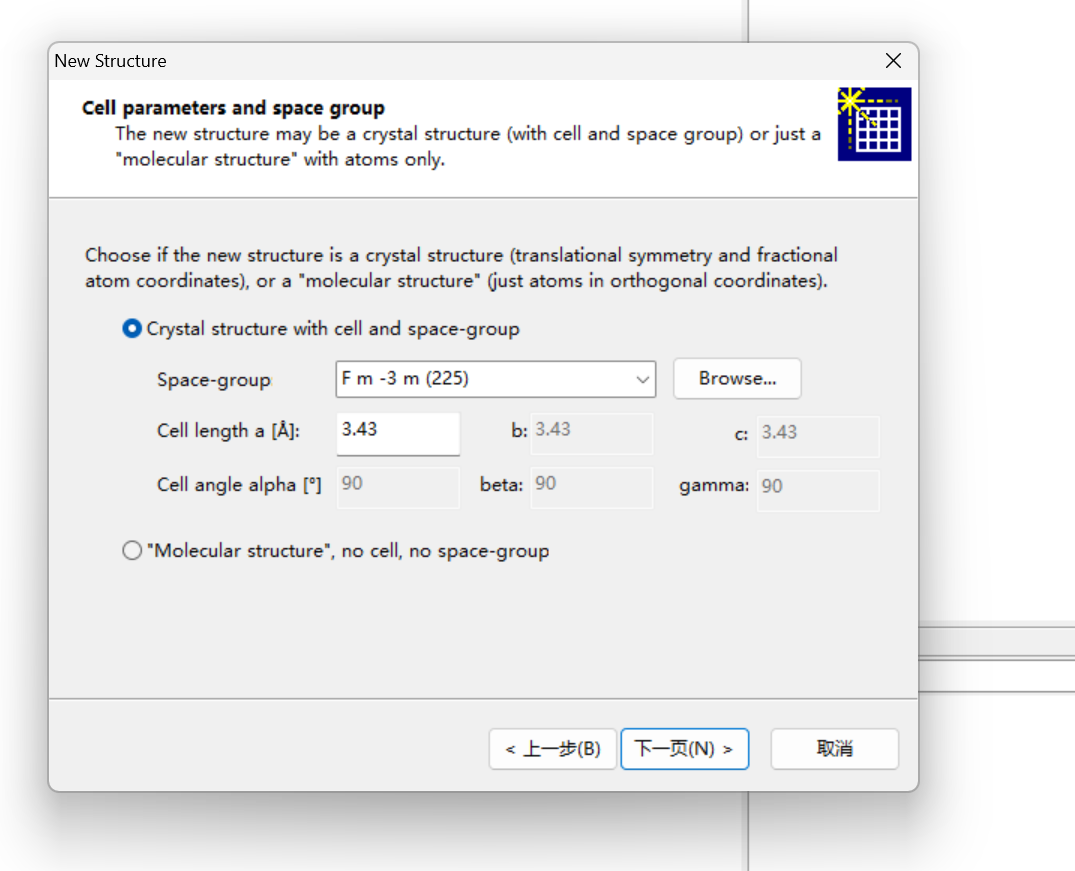
\includegraphics[width=0.44\textwidth]{assets/fcc/a.png}}
  \hfill
  \subcaptionbox{非对称单元原子（Fe）添加}{%
    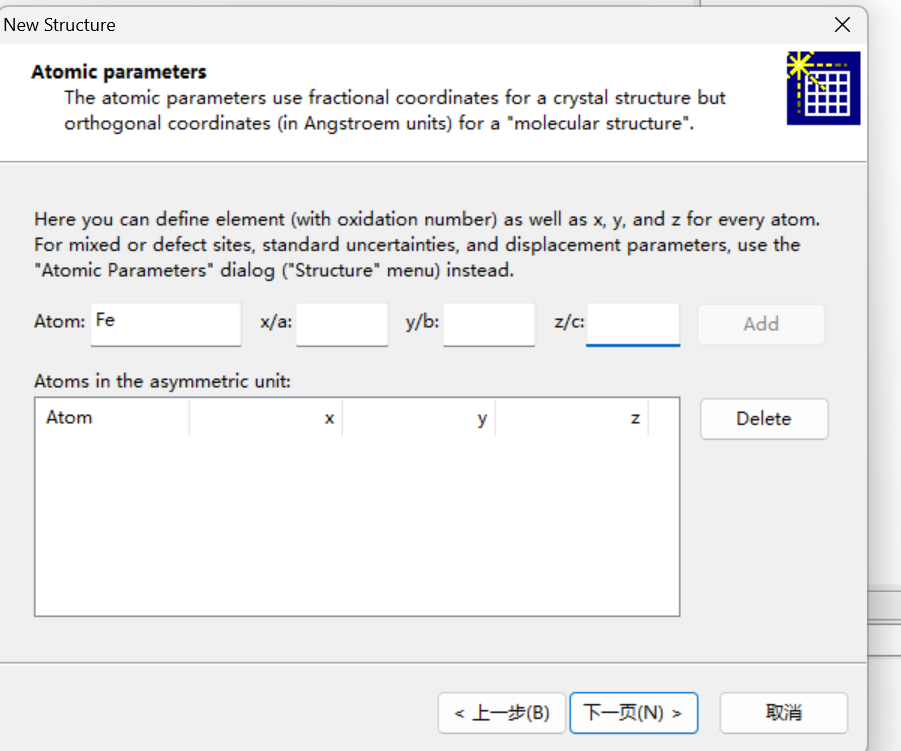
\includegraphics[width=0.44\textwidth]{assets/fcc/b.png}}
  \caption{面心立方（FCC）结构的参数设置}
  \label{fig:fcc-param}
\end{figure}

\begin{figure}[H]
  \centering
  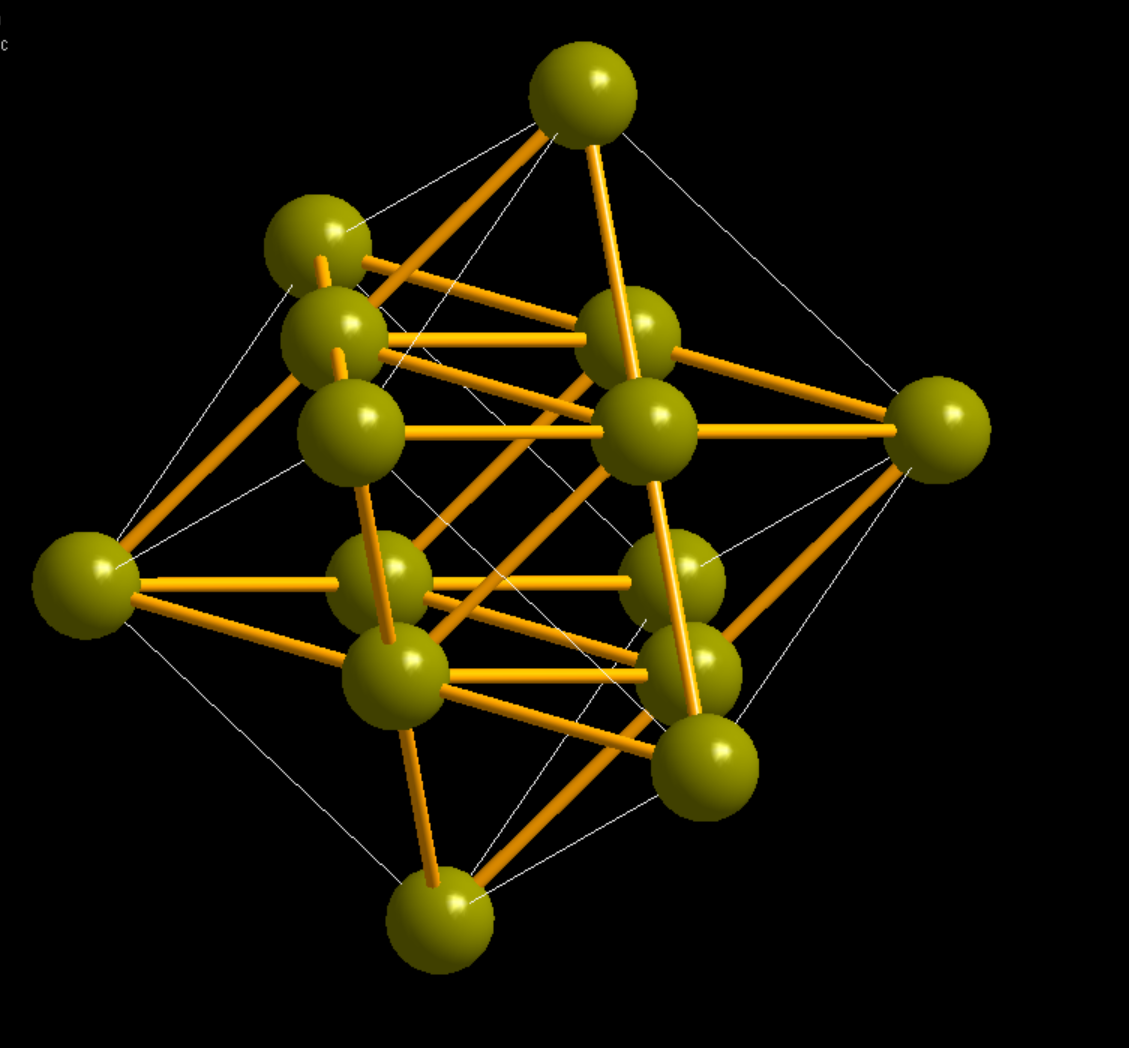
\includegraphics[width=0.5\textwidth]{assets/fcc/c.png}
  \caption{面心立方（FCC）结构的晶体结构模型}
  \label{fig:fcc-model}
\end{figure}

\begin{figure}[H]
  \centering
  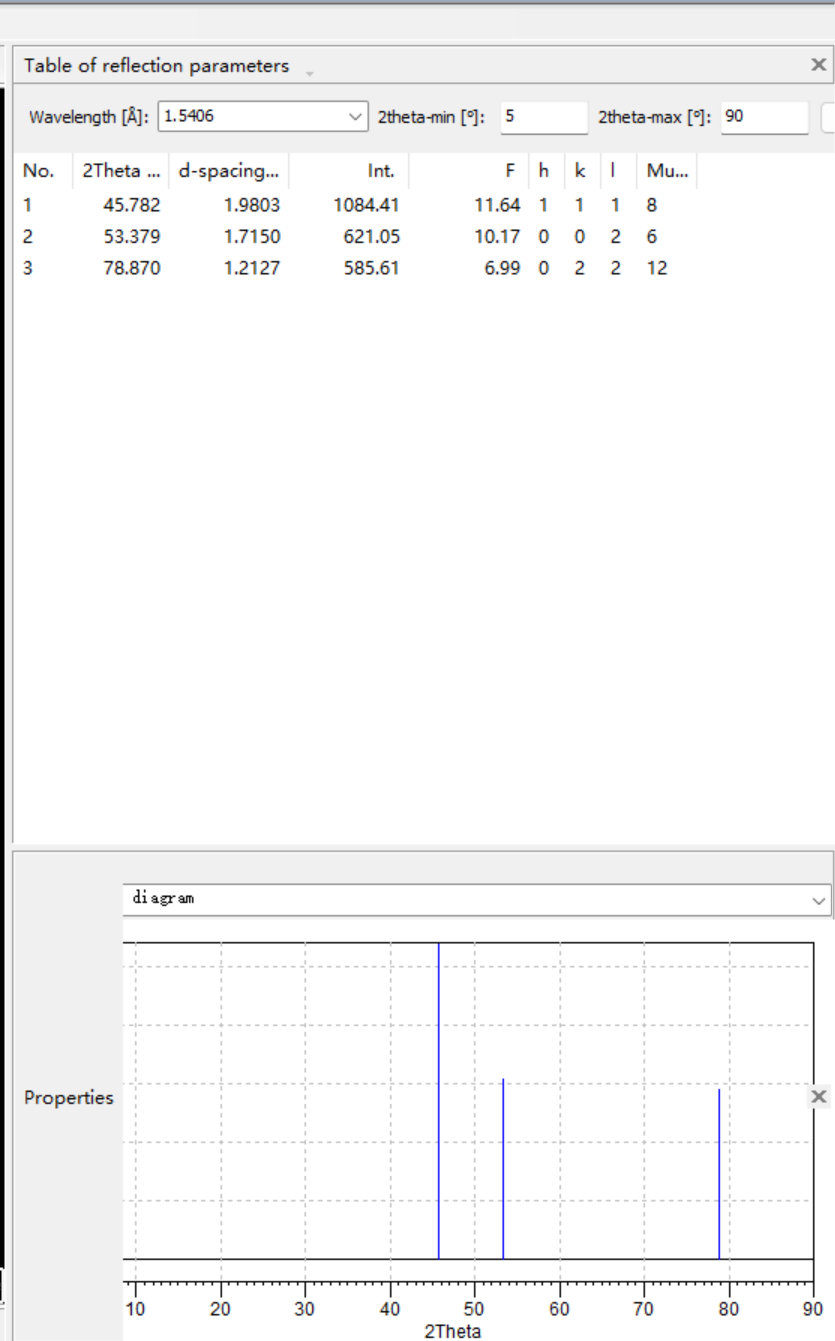
\includegraphics[width=0.4\textwidth]{assets/fcc/d.png}
  \caption{Diamond 模拟的面心立方（FCC）结构粉末衍射图}
  \label{fig:fcc-xrd}
\end{figure}

\begin{figure}[H]
  \centering
  \subcaptionbox{$\{111\}$ 密排面视图}{%
    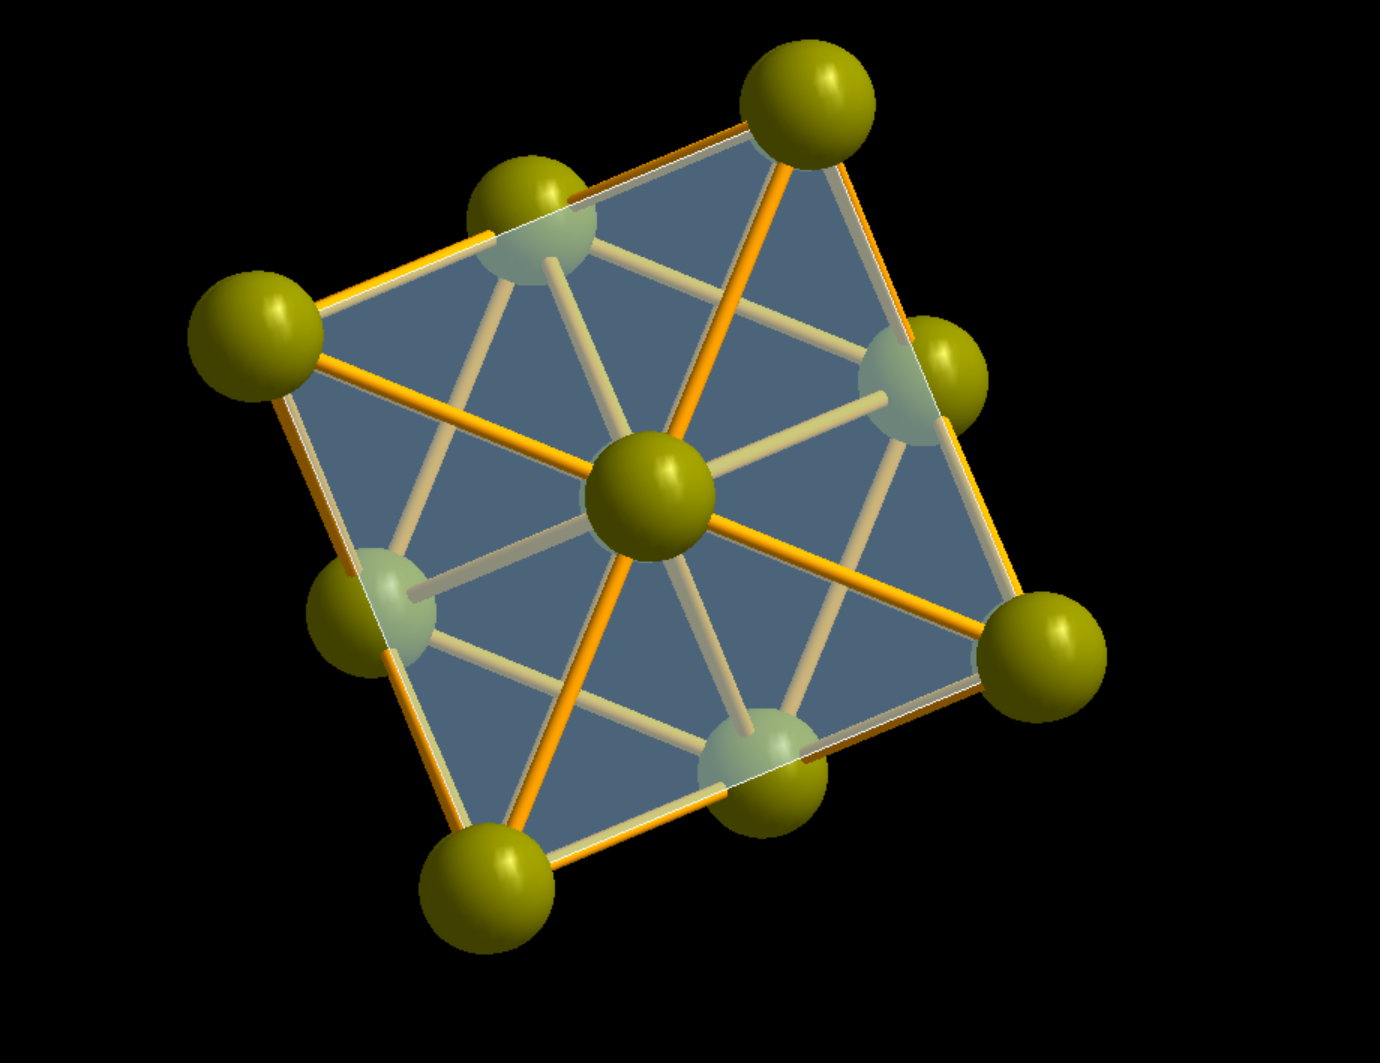
\includegraphics[width=0.46\textwidth]{assets/fcc/e.png}}
  \hfill
  \subcaptionbox{最近邻配位多面体（配位数 12）}{%
    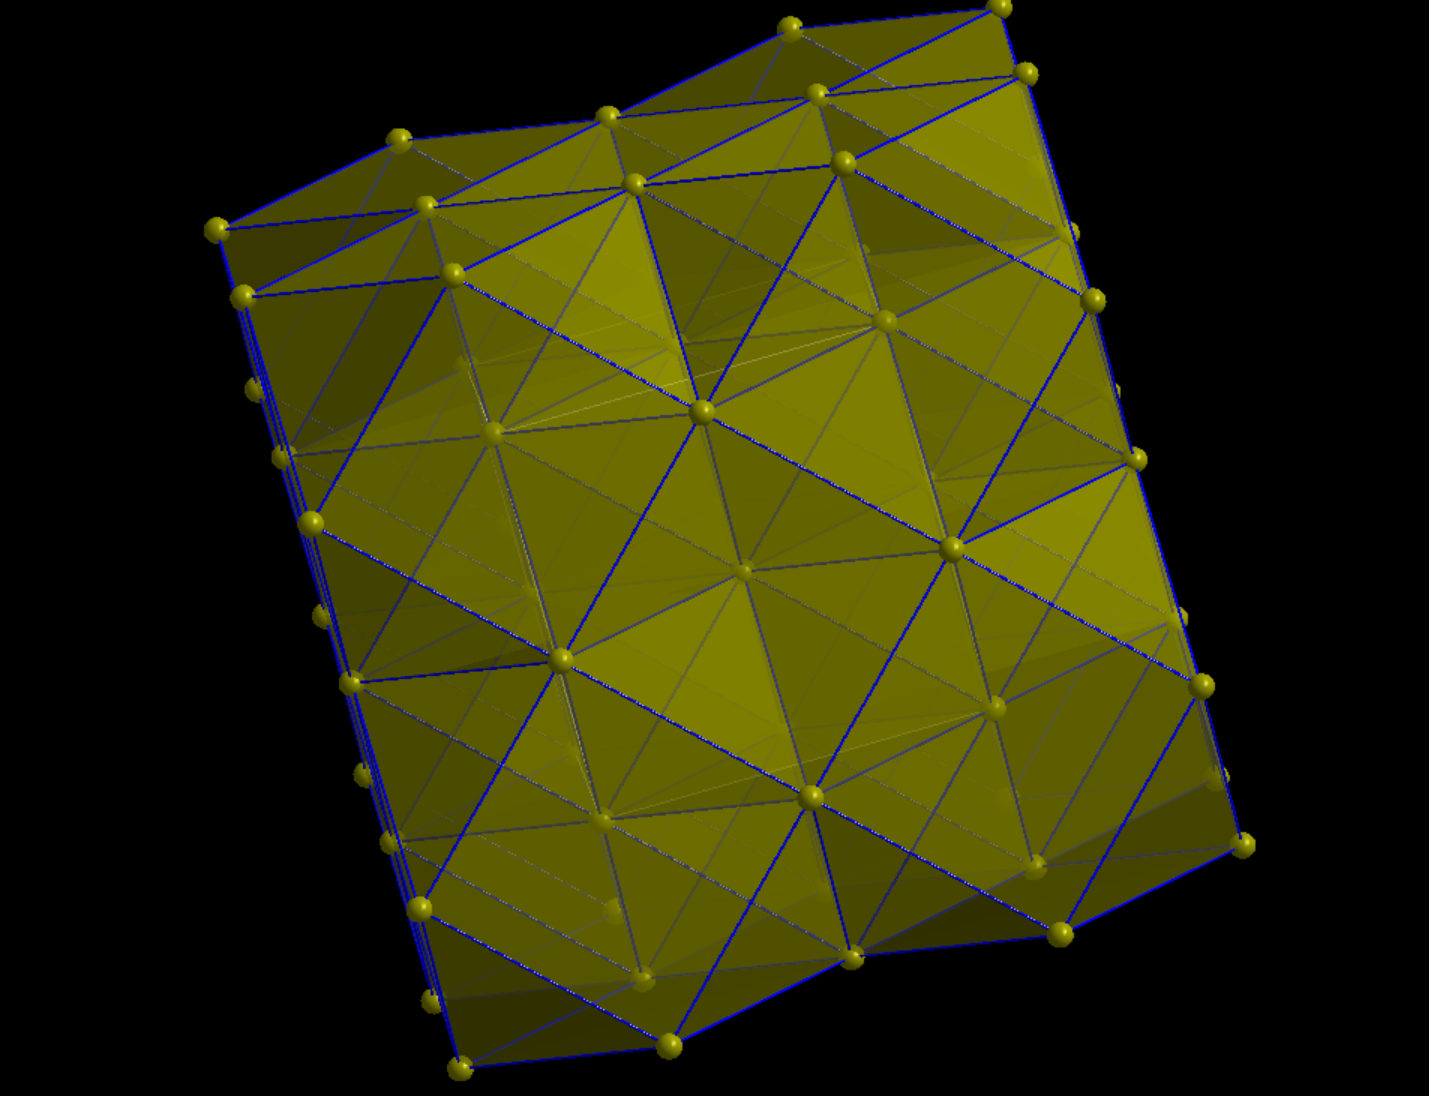
\includegraphics[width=0.44\textwidth]{assets/fcc/f.png}}
  \caption{面心立方（FCC）结构的密排面与配位多面体}
  \label{fig:fcc-plane}
\end{figure}

\textbf{结构特征。}面心立方晶胞的原子位于 8 个顶点与 6 个面心：顶点各计 $1/8$、面心各计
$1/2$，折合晶胞内共 $8\times1/8+6\times1/2=4$ 个原子（图~\ref{fig:fcc-model}）。

FCC 的密排方向为面对角线方向 $\langle110\rangle$。沿面对角线，两端的面心原子与中间的
顶点原子相切，故 $4r=\sqrt{2}a$，即原子半径 $r=\sqrt{2}a/4$；代入本次建模所用的
$a=3.43$\,\AA 得 $r\approx1.21$\,\AA。每个原子的最近邻有 12 个（同层 6 个、上下层各
3 个），次近邻 6 个（沿 $\langle100\rangle$ 方向），最近邻配位多面体是立方八面体
（图~\ref{fig:fcc-plane}(b)）。把 4 个原子的体积与晶胞体积相比，得原子堆积因子
\begin{equation}
  \eta=\frac{4\times\frac{4}{3}\pi r^3}{a^3}
    =\frac{4\times\frac{4}{3}\pi\left(\frac{\sqrt{2}}{4}a\right)^3}{a^3}
    =\frac{\sqrt{2}\pi}{6}\approx0.7405
\end{equation}
与 HCP 并列为最紧密的堆积方式。密排面为 $\{111\}$ 面（图~\ref{fig:fcc-plane}(a)），
密排层沿 $\langle111\rangle$ 方向按 ABCABC 顺序交替堆积。晶胞内的间隙同样可以清点：
八面体间隙 4 个，位于体心 $(1/2,1/2,1/2)$ 及各棱中点；四面体间隙 8 个，如
$(1/4,1/4,1/4)$。

在 $F\,m\,\bar3\,m$ 这一符号里，$F$ 表示面心点阵，后面三个特征方向依次对应 [100] 的
镜面 $m$、[111] 的旋转反演轴 $\bar3$（立方晶系的标志）和 [110] 的镜面 $m$。Cu、Ag、Au、
Al、Ni 与 $\gamma$-Fe 都具有 FCC 结构，NaCl、金刚石等结构也以 FCC 点阵为基础。
